% Formal Verification of Quantum Codes with Transversal Diagonal Gates
% Compile with: xelatex distance2_talk.tex
\documentclass[aspectratio=169,t]{beamer}
\usetheme{metropolis}
\metroset{
  progressbar=frametitle,
  sectionpage=progressbar,
  numbering=fraction,
  block=fill,
}

% ── Fonts (XeLaTeX) ──────────────────────────────────────────────────
\usepackage{fontspec}
\setsansfont{FiraSans}[
  Extension=.otf,
  Path=/opt/homebrew/Cellar/texlive/20250308_2/share/texmf-dist/fonts/opentype/public/fira/,
  UprightFont=*-Regular,
  BoldFont=*-SemiBold,
  ItalicFont=*-Italic,
  BoldItalicFont=*-SemiBoldItalic,
]
\setmonofont{FiraMono}[
  Extension=.otf,
  Path=/opt/homebrew/Cellar/texlive/20250308_2/share/texmf-dist/fonts/opentype/public/fira/,
  UprightFont=*-Regular,
  BoldFont=*-Bold,
  Scale=0.85,
]

% ── Packages ─────────────────────────────────────────────────────────
\usepackage{amsmath,amssymb}
\usepackage{braket}
\usepackage{booktabs}
\usepackage{colortbl}
\usepackage{tikz}
\usetikzlibrary{arrows.meta,positioning,fit,calc,shapes,decorations.markings}
\usepackage{listings}
\usepackage{xcolor}

% ── Color Palette ────────────────────────────────────────────────────
\definecolor{Navy}{HTML}{1B2A4A}
\definecolor{Teal}{HTML}{0D7377}
\definecolor{Coral}{HTML}{E85D4A}
\definecolor{Amber}{HTML}{E8A838}
\definecolor{Sage}{HTML}{2D8F5E}
\definecolor{Slate}{HTML}{4A5568}
\definecolor{Ice}{HTML}{E8F4F8}
\definecolor{LeanBG}{HTML}{F0F4F8}
\definecolor{LeanBlue}{HTML}{1A3A6B}
\definecolor{LeanKW}{HTML}{0D5E8C}
\definecolor{LeanStr}{HTML}{1D7A4E}

% ── Metropolis Color Customization ───────────────────────────────────
\setbeamercolor{frametitle}{bg=Navy, fg=white}
\setbeamercolor{progress bar}{fg=Coral, bg=Navy!20}
\setbeamercolor{title separator}{fg=Coral}
\setbeamercolor{alerted text}{fg=Coral}
\setbeamercolor{example text}{fg=Teal}
\setbeamercolor{block title}{bg=Teal!85!black, fg=white}
\setbeamercolor{block body}{bg=Teal!8}
\setbeamercolor{block title alerted}{bg=Coral!85!black, fg=white}
\setbeamercolor{block body alerted}{bg=Coral!6}
\setbeamercolor{block title example}{bg=Sage!80!black, fg=white}
\setbeamercolor{block body example}{bg=Sage!6}
\setbeamercolor{section in toc}{fg=Navy}
\setbeamercolor{normal text}{fg=Navy!90!black}

% ── Lean listing style ───────────────────────────────────────────────
\lstdefinestyle{lean}{
  language={},
  basicstyle=\ttfamily\small,
  keywordstyle=\color{LeanKW}\bfseries,
  commentstyle=\color{Slate}\itshape,
  stringstyle=\color{LeanStr},
  morekeywords={theorem,def,structure,where,by,native_decide,import,open,
    instance,lemma,example,abbrev,noncomputable,section,end,namespace,
    Decidable,Prop,Bool,true,Fin,Finset,ZMod,BitString},
  backgroundcolor=\color{LeanBG},
  frame=l,
  framerule=2pt,
  rulecolor=\color{Teal},
  xleftmargin=8pt,
  xrightmargin=4pt,
  aboveskip=6pt,
  belowskip=4pt,
  breaklines=true,
  columns=fullflexible,
  literate={→}{{$\to$}}1 {∀}{{$\forall$}}1 {∈}{{$\in$}}1 {≤}{{$\leq$}}1
           {≥}{{$\geq$}}1 {≠}{{$\neq$}}1 {∑}{{$\sum$}}1 {ψ}{{$\psi$}}1
           {₀}{{$_0$}}1 {₁}{{$_1$}}1 {ℚ}{{$\mathbb{Q}$}}1
           {:=}{{$\,:=\,$}}2 {=>}{{$\Rightarrow$}}1,
}

% ── Custom commands ──────────────────────────────────────────────────
\newcommand{\ZZ}{\mathbb{Z}}
\newcommand{\QQ}{\mathbb{Q}}
\newcommand{\CC}{\mathbb{C}}
\newcommand{\Fintwo}{\{0,1\}}
\newcommand{\wt}{\mathrm{wt}}
\newcommand{\code}[1]{\texttt{\small #1}}
\newcommand{\chk}{\textcolor{Sage}{\checkmark}}
\newcommand{\leanproof}{ \textcolor{Sage}{\checkmark\,\texttt{native\_decide}}}

% ── TikZ global styles ──────────────────────────────────────────────
\tikzset{
  pipebox/.style={draw=Navy!60, rounded corners=5pt, minimum height=1cm,
    text width=3.6cm, align=center, font=\small,
    fill=#1},
  pipebox/.default={white},
  fatarr/.style={-{Stealth[length=6pt,width=5pt]}, thick, color=Teal!80!black},
}

% ── Title ────────────────────────────────────────────────────────────
\title{Formal Verification of Quantum Codes\\
  with Transversal Diagonal Gates in Lean~4}
\author{\textbf{Sirui Lu} \and Xi He \and Bei Zeng}
\institute{University of Texas at Dallas}
\date{2026}

\begin{document}

% =====================================================================
% TITLE
% =====================================================================
{
\setbeamercolor{background canvas}{bg=Navy}
\setbeamercolor{normal text}{fg=white}
\usebeamercolor[fg]{normal text}
\begin{frame}[plain,noframenumbering]
\vfill
\begin{center}
{\Large\bfseries\textcolor{white}{Formal Verification of Quantum Codes}\\
\textcolor{white}{with Transversal Diagonal Gates in Lean~4}}

\vspace{1.2em}
%{\normalsize\textcolor{Ice}{Sirui Lu \;\;$\cdot$\;\; Xi He \;\;$\cdot$\;\; Bei Zeng}}\\
{\small\textcolor{Teal!60!white}{University of Texas at Dallas}}

\vspace{1.5em}
{\footnotesize\textcolor{Slate!40!white}{%
  arXiv:2510.20728 \quad$\cdot$\quad
  \texttt{github.com/LionSR/lean-qec}}}
\end{center}
\vfill
\end{frame}
}

% =====================================================================
% OUTLINE
% =====================================================================
\begin{frame}{Outline}
\tableofcontents[hideallsubsections]
\end{frame}

% =====================================================================
% Slide: This Talk
% =====================================================================
\begin{frame}{This Talk}

\textbf{Starting point}: arXiv:2510.20728 catalogued \alert{14,116} distance-2 codes
with transversal diagonal gates via the SSLP pipeline.

\vspace{0.2em}
\textbf{Three new contributions}:
\begin{enumerate}\setlength\itemsep{1pt}
\item \textbf{Lean~4 formalization} of the full SSLP pipeline ---
  machine-checked proofs, zero \code{sorry}
\item \textbf{Analytical families}: one proof covers \emph{infinitely many} codes
\item \textbf{Distance-3 generalization}: exact solutions for $((7,2,3))$ codes
  discovered by \alert{GPT-5.2}, formally verified in Lean
\end{enumerate}

\vspace{0.3em}
\begin{center}
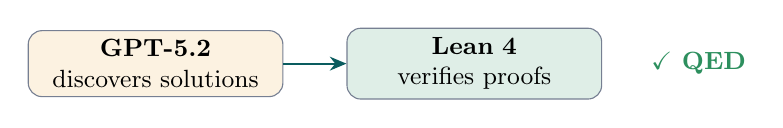
\begin{tikzpicture}
  \node[pipebox=Amber!15, text width=3cm, minimum height=0.7cm, font=\small]
    (ai) {\textbf{GPT-5.2}\\discovers solutions};
  \node[pipebox=Sage!15, text width=3cm, minimum height=0.7cm, font=\small, right=0.8cm of ai]
    (lean) {\textbf{Lean 4}\\verifies proofs};
  \draw[fatarr] (ai) -- (lean);
  \node[right=0.5cm of lean, font=\small\bfseries, text=Sage] {$\checkmark$ QED};
\end{tikzpicture}
\end{center}
\end{frame}

% =====================================================================
\section{Transversal Gates \& the SSLP Pipeline}
% =====================================================================

% =====================================================================
% Slide: Transversal Diagonal Gates
% =====================================================================
\begin{frame}{Transversal Diagonal Gates}

\textbf{Physical gate} with angle vector
$\mathbf{a}=(a_1,\ldots,a_n)\in\ZZ_m^n$:
\[
  U(\mathbf{a},m)
  = 
  \bigotimes_{i=1}^{n}\!
  \begin{pmatrix}1&0\\0&\omega_m^{a_i}\end{pmatrix},
  \qquad
  \omega_m = e^{2\pi i/m}
\]

Action on computational basis:
$ U(\mathbf{a},m)\ket{x}
  =  \omega_m^{\,\langle\mathbf{a},\,x\rangle}\ket{x}$
where
$\langle\mathbf{a},x\rangle
  = \sum_{i} a_i\, x_i$.

Define \textbf{residue classes}
$ C_b(\mathbf{a})
  = 
  \bigl\{x\in\Fintwo^n :
    \sum_i a_i x_i \equiv b \pmod{m}\bigr\}$.

\begin{alertblock}{Eigenstate condition}
$\mathrm{supp}(\ket{j_L})\subseteq C_{S_j}(\mathbf{a})
  \Longrightarrow  
U(\mathbf{a},m)\ket{j_L} = \omega_m^{S_j}\ket{j_L}$
\end{alertblock}
\end{frame}

% =====================================================================
% Slide: SSLP Pipeline
% =====================================================================
\begin{frame}{The SSLP Pipeline
  \hfill{\footnotesize\textcolor{Slate}{[Zhang--Zeng, 2504.20847]}}}

\textbf{S}ubset-\textbf{S}um \textbf{L}inear \textbf{P}rogramming:
systematic code construction.

\vspace{0.5em}
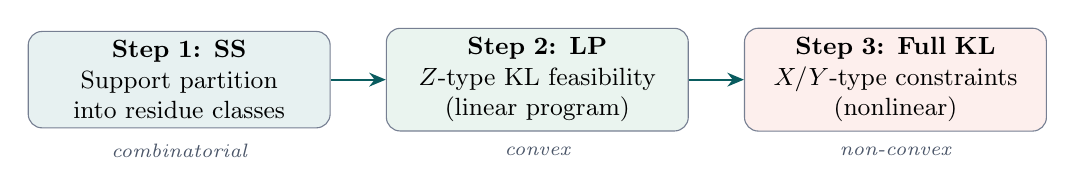
\begin{tikzpicture}
  \node[pipebox=Teal!10]  (ss)   {\textbf{Step 1: SS}\\Support partition\\into residue classes};
  \node[pipebox=Sage!10,  right=0.7cm of ss]  (lp)
    {\textbf{Step 2: LP}\\$Z$-type KL feasibility\\(linear program)};
  \node[pipebox=Coral!10, right=0.7cm of lp]  (full)
    {\textbf{Step 3: Full KL}\\$X/Y$-type constraints\\(nonlinear)};

  \draw[fatarr] (ss) -- (lp);
  \draw[fatarr] (lp) -- (full);

  \node[below=2pt of ss, font=\scriptsize\itshape, text=Slate]
    {combinatorial};
  \node[below=2pt of lp, font=\scriptsize\itshape, text=Slate]
    {convex};
  \node[below=2pt of full, font=\scriptsize\itshape, text=Slate]
    {non-convex};
\end{tikzpicture}

\vspace{0.3em}
Step~2 is an LP $\Rightarrow$ fast rejection of infeasible parameters.

For \alert{distance~2}: our residue-shift screen makes Step~3 \emph{automatic}.

For \alert{distance~3}: we solve Step~3 via exact arithmetic in $\QQ(\sqrt2,\sqrt3,i)$.
\end{frame}

% =====================================================================
% Slide: SS Step
% =====================================================================
\begin{frame}{Step 1: Subset-Sum Support Partition}

Residue classes
$C_b(\mathbf{a})
  = 
  \bigl\{x\in\Fintwo^n :
    \sum_i a_i x_i \equiv b \pmod{m}\bigr\}$
partition $\Fintwo^n$.

\begin{columns}[T]
\column{0.52\textwidth}
\begin{itemize}
\item \textbf{Disjoint}: $C_b\cap C_{b'} = \emptyset$ for $b\neq b'$
  $ \Rightarrow$ automatic orthogonality
\item \textbf{Logical action}:
  $U\ket{j_L} = \omega_m^{S_j}\ket{j_L}$
\item \textbf{Projective order}:
  $\mathcal{O} = m\,/\,\gcd(m,S_1-S_0,\ldots)$
\end{itemize}

\column{0.44\textwidth}
\begin{exampleblock}{Example: $n{=}5$, $m{=}7$}
$\mathbf{a}{=}(1,1,2,2,2)$, $(S_0,S_1)=(0,4)$

$C_0 = \{00000, 01111, 10111\}$

$C_4 = \{00011, 00101, \ldots\}$ (6 elts)

$\mathcal{O}=7/\gcd(7,4)=7$
\end{exampleblock}
\end{columns}
\end{frame}

% =====================================================================
% Slide: Z-type KL as LP
% =====================================================================
\begin{frame}{Step 2: $Z$-Type KL as Linear Program}

Probabilities $p_{j,x}=|c_{j,x}|^2$ on support of $\ket{j_L}$.

\textbf{$Z$-type KL}: $\braket{j_L|Z_i|j_L}=t_i$ independent of $j$ becomes
\[
  \boxed{ \sum_{x\in C_{S_j}}\! (-1)^{x_i}\, p_{j,x} =  t_i
  \qquad\forall\, i\in[n], \forall\, j }
\]

\begin{columns}[T]
\column{0.48\textwidth}
\textbf{Linear} in $p_{j,x}$ with constraints:
\begin{itemize}
\item $\sum_{x\in C_{S_j}} p_{j,x} = 1$
\item $p_{j,x} \geq 0$
\end{itemize}
Standard LP feasibility.

\column{0.48\textwidth}
\textbf{Geometric view}: sign vectors
$v(x)=((-1)^{x_1},\ldots,(-1)^{x_n})$
are vertices.

Feasibility $=$ nonempty
$\bigcap_{j}\mathrm{conv}(V_j)$.
\end{columns}
\end{frame}

% =====================================================================
% Slide: Residue-Shift Screen
% =====================================================================
\begin{frame}{Residue-Shift Screen: Distance 2 for Free}

Flipping bit $i$ shifts the residue by $\pm a_i$:
\[
  \langle\mathbf{a},\, x\oplus e_i\rangle
  \equiv 
  \langle\mathbf{a},\, x\rangle \pm a_i \pmod{m}
\]

\begin{alertblock}{Residue-Shift Screen}
$S_j - S_k \not\equiv \pm a_i \pmod{m}$ 
for all $i\in[n]$, all $j\neq k$
$  \Longrightarrow  $
union support has $d_H \geq 2$.
\end{alertblock}

When the screen passes, \alert{all $X/Y$-type KL vanish automatically}.

\begin{center}
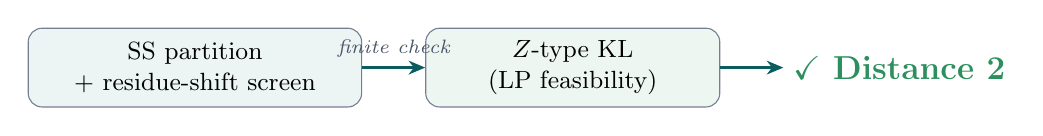
\begin{tikzpicture}
  \node[pipebox=Teal!8, text width=4cm]  (a) {SS partition\\+ residue-shift screen};
  \node[pipebox=Sage!8, text width=3.5cm, right=0.8cm of a]  (b) {$Z$-type KL\\(LP feasibility)};
  \node[right=0.8cm of b, font=\large\bfseries, text=Sage] (c)
    {$\checkmark$ Distance 2};

  \draw[fatarr] (a) -- node[above, font=\scriptsize\itshape, text=Slate]{finite check} (b);
  \draw[fatarr] (b) -- (c);
\end{tikzpicture}
\end{center}
\end{frame}

% =====================================================================
% Slide: BD Symmetry
% =====================================================================
\begin{frame}{Binary Dihedral Symmetry ($K{=}2$)}

\begin{columns}[T]
\column{0.52\textwidth}
Binary dihedral group $\mathrm{BD}_{2m}$:
\begin{itemize}
\item Generated by $Z(2\pi/m)$ and $\hat{X}=-iX$
\item $|\mathrm{BD}_{2m}|=4m$;\quad $m{=}8 \Rightarrow$ transversal $T$
\item Transversal $\overline{X}=X^{\otimes n}$: 
  $\ket{1_L} = X^{\otimes n}\ket{0_L}$
\item Support: $S_1 = \bar{S}_0$  (bitwise complements)
\item Amplitudes: $c_{1,\bar{x}}=c_{0,x}$
\end{itemize}

\column{0.44\textwidth}
\begin{block}{BD angle condition}
$\sum_{j=1}^{n} a_j \equiv  -1 \pmod{m}$
\end{block}

\begin{exampleblock}{$Z$-balance}
Complement symmetry forces\\
$\sum_{x\in S_0}(-1)^{x_i}p_x = 0$
for all $i$.

Only $\ket{0_L}$ needs specification.
\end{exampleblock}
\end{columns}
\end{frame}

% =====================================================================
\section{Distance-2 Results}
% =====================================================================

% =====================================================================
% Slide: Catalogue
% =====================================================================
\begin{frame}{Catalogue: 14,116 Distance-2 Codes
  \hfill{\footnotesize\textcolor{Slate}{[arXiv:2510.20728]}}}

\begin{columns}[T]
\column{0.50\textwidth}
Systematic search via SSLP:
\begin{itemize}\setlength\itemsep{1pt}
\item $K\in\{2,3,4\}$, $n\leq 6$, $m\leq 18$
\item Residue-shift screen for $d{=}2$
\item LP solver + rational reconstruction
\end{itemize}

\begin{center}
{\Huge\textcolor{Coral}{\textbf{14,116}}}\\
certified $((n,K,2))$ codes
\end{center}

\column{0.46\textwidth}
\begin{block}{Highlights}
\begin{itemize}\setlength\itemsep{1pt}
\item Orders $\mathcal{O}=2$ through $18$ at $n=6$
\item Mostly \textbf{nonadditive}
\item Includes $K=3,4$ codes
\end{itemize}
\end{block}

\begin{exampleblock}{Analytical families}
Family I: $C_0=\{0^n,1^n\}$,\\
closed-form $p(0^n)=1-s/m$\\
\chk  verified in Lean for all $(n,m,s)$
\end{exampleblock}
\end{columns}
\end{frame}

% =====================================================================
% Slide: Analytical Families
% =====================================================================
\begin{frame}{Analytical Families: One Proof, Infinitely Many Codes}

Find a \textbf{closed-form pattern}, prove it \emph{once}, instantiate everywhere.

\begin{columns}[T]
\column{0.50\textwidth}
\begin{block}{Family I: the simplest codes}
Support $C_0 = \{0^n, 1^n\}$ --- just two basis states.

$\ket{0_L} = \sqrt{p}\,\ket{0\cdots 0} + \sqrt{1{-}p}\,\ket{1\cdots 1}$

$Z$-balance forces $p$ \textbf{uniquely}: $p = 1 - s/m$.

Valid for \emph{all} $(n,m,\mathbf{a})$ passing the screen.
\end{block}

\column{0.46\textwidth}
\begin{exampleblock}{$\lambda$-families}
Larger supports, free parameter $\lambda$:
\begin{itemize}\setlength\itemsep{0pt}
\item $\lambda$-Family II: $|C_0|=4$
\item $\lambda$-Family V: $|C_0|=6$
\item 5 families, each a \textbf{universally\\
  quantified} Lean theorem
\end{itemize}
\end{exampleblock}

\tikz\node[draw=Sage, fill=Sage!6, rounded corners=3pt, inner sep=4pt, text width=4cm, align=center, font=\small]{%
  One Lean proof $\Leftrightarrow$\\infinitely many verified codes};
\end{columns}
\end{frame}

% =====================================================================
% Slide: Worked Example
% =====================================================================
\begin{frame}[fragile]{Worked Example: $((5,2,2))$ Code}

$n{=}5$, $\mathbf{a}{=}(1,1,2,2,2)$, $m{=}7$, $(S_0,S_1)=(0,4)$

\begin{columns}[T]
\column{0.48\textwidth}

\textbf{SS}: 
$C_0 = \{00000,  01111,  10111\}$, 
$C_4$: 6 elements

\textbf{Screen}: 
$4 \not\equiv  \pm 1, \pm 2 \pmod{7}$ \chk

\textbf{LP}: 
$p_{00000}=3/7$, 
$p_{01111}=p_{10111}=2/7$

$\braket{Z_i} = 3/7$ ($i{=}1,2$), 
$-1/7$ ($i{=}3,4,5$)

\column{0.48\textwidth}
\begin{exampleblock}{Lean: one-line proof}
\begin{lstlisting}[style=lean,basicstyle=\ttfamily\footnotesize]
def myCode : ExampleData where
  n := 5;  m := 7;  K := 2
  a := ![1, 1, 2, 2, 2]
  S := ![0, 4]
  supp := ![supp0, supp1]
  prob := ![prob0, prob1]

theorem verified : myCode.OK :=
  by native_decide
\end{lstlisting}
\end{exampleblock}
\end{columns}

\vspace{0.1em}
\begin{center}
\tikz\node[draw=Sage, fill=Sage!6, rounded corners=3pt, inner sep=4pt]{%
  \textbf{SS $+$ screen $+$ LP} $ \Rightarrow $
  certified $((5,2,2))$ code, order $\mathcal{O}=7$.\;
  Build: ${<}\,1$\,s.
};
\end{center}
\end{frame}

% =====================================================================
\section{Lean~4 Formalization}
% =====================================================================

% =====================================================================
% Slide: What is Lean 4?
% =====================================================================
\begin{frame}{What is Lean~4?}

\begin{columns}[T]
\column{0.55\textwidth}
A \textbf{proof assistant} based on dependent type theory:
\begin{itemize}\setlength\itemsep{0pt}
\item Every proof is a program; the \textbf{kernel} type-checks it
\item Compiles $\Rightarrow$ proof is correct.  No trust required.
\item \textbf{Mathlib}: 180K+ formalized theorems
\end{itemize}

\textbf{Key tactic}: \code{native\_decide}
\begin{itemize}\setlength\itemsep{0pt}
\item Proposition is \code{Decidable}?
  Compile to native code $\to$ run $\to$ \code{true}
\item Kernel accepts: proof complete
\item ``All 49,152 KL constraints hold?''
  $\to$ \code{true} $\to$ QED
\end{itemize}

\column{0.42\textwidth}
\begin{exampleblock}{Landmark projects}
\begin{itemize}\setlength\itemsep{0pt}
\item Freiman--Ruzsa conj.\ (Tao)
\item Liquid Tensor Experiment
\item Sphere eversion
\item \alert{This work}: quantum codes
\end{itemize}
\end{exampleblock}

\begin{block}{Why Lean for QEC?}
14K codes: too many for humans.\\
AI-found solutions: trust but verify.\\
Formal proof $=$ \textbf{certainty}.
\end{block}
\end{columns}
\end{frame}

% =====================================================================
% Slide: Architecture
% =====================================================================
\begin{frame}{Lean~4 Codebase: \texttt{lean-qec}}

\begin{columns}[T]
\column{0.30\textwidth}
{\small\textbf{Core Library (\code{SS/})}}\\
\code{BitString.lean}\\
\code{Basic.lean}\\
\code{DiagonalAction.lean}\\
\code{ResidueShiftScreen.lean}\\
\code{ZTypeKL.lean}\\
\code{BDSymmetry.lean}\\
\code{Verify.lean}\\
\code{FamilyI/} \textcolor{Slate}{\scriptsize(6 files)}\\
\code{LambdaV2/} \textcolor{Slate}{\scriptsize(5 families)}

\column{0.30\textwidth}
{\small\textbf{Distance-3 Modules}}\\
\code{Pauli.lean}\\
\code{FullKL.lean}\\
\code{QSqrt23i.lean}\\
\code{FullKLEval.lean}\\
\code{Distance3Verify.lean}\\
\code{BD16Defs.lean}


{\small\textbf{Codebase}}\\
${\sim}$4,300 lines, ${\sim}$30 modules\\
0 \code{sorry},  0 warnings

\column{0.36\textwidth}
{\small\textbf{Examples}}\\
\code{Examples/D2/}\\
\quad\code{Ex522.lean} \textcolor{Slate}{\scriptsize $((5,2,2))$}\\
\quad\code{Ex622.lean} \textcolor{Slate}{\scriptsize $((6,2,2))$}\\
\code{Examples/D3/}\\
\quad\code{BD16v1.lean} \textcolor{Slate}{\scriptsize through}\\
\quad\code{BD16v6a.lean} \textcolor{Slate}{\scriptsize (8 codes)}\\
{\small\textbf{Build}}\\
3,091 jobs\\
\textcolor{Sage}{\textbf{0 errors $\cdot$ 0 warnings}}
\end{columns}
\end{frame}

% =====================================================================
% Slide: Formalization Highlights
% =====================================================================
\begin{frame}[fragile]{Formalization: Key Theorems}

\begin{columns}[T]
\column{0.48\textwidth}
\begin{block}{\code{Dact\_eq\_global\_of\_SS}}
$\mathrm{supp}(\ket{j_L})\subseteq C_{S_j}
 \Rightarrow 
U\ket{j_L} = \omega_m^{S_j}\ket{j_L}$
\end{block}

\begin{block}{\code{no\_hamming1\_neighbor\_of\_screen}}
Screen condition $\Rightarrow$
$d_H(x,y)\geq 2$ across classes\\
$\Rightarrow$ all $X/Y$-type KL vanish
\end{block}

\column{0.48\textwidth}
\begin{alertblock}{\code{ExampleData.OK}}
Bundles four checks:
\begin{enumerate}\setlength\itemsep{0pt}
\item SS support condition
\item Residue-shift screen
\item Probability normalization
\item $Z$-type KL matching
\end{enumerate}
All \code{Decidable} $\Rightarrow$\\
\code{native\_decide} in $<1$\,s
\end{alertblock}
\end{columns}

\vspace{0.5em}
\textbf{Technique}: \code{BitString n} $= \texttt{Fin} n \to \texttt{Bool}$ has $2^n$ elements.
All quantifiers over finite support are decidable $\Rightarrow$ 
Lean compiles to native code, executes, returns \code{true} $\Rightarrow$ kernel accepts as proof.
\end{frame}

% =====================================================================
\section{Distance-3 Extension}
% =====================================================================

% =====================================================================
% Slide: The Distance-3 Barrier
% =====================================================================
\begin{frame}{The Distance-3 Barrier}

\begin{columns}[T]
\column{0.48\textwidth}
\textbf{Why was distance 2 ``easy''?}
\begin{itemize}\setlength\itemsep{1pt}
\item Residue-shift screen kills all $X/Y$-type KL automatically
\item Only $Z$-type survives $\Rightarrow$ linear in probabilities $p_x \geq 0$
\item \alert{No complex amplitudes needed}
\end{itemize}

\column{0.48\textwidth}
\textbf{Why is distance 3 harder?}
\begin{itemize}\setlength\itemsep{1pt}
\item Must check all weight-${\leq}\,2$ Paulis:
  $Z_iZ_j, X_iX_j, X_iY_j, \ldots$
\item $X,Y$ \textbf{flip bits} $\Rightarrow$ couples different
  basis states
\item KL becomes \textbf{quadratic} in $c_x \in \CC$
\item \alert{Relative phases matter}
\end{itemize}
\end{columns}

\vspace{0.5em}
\textbf{The gap}: distance-2 $=$ convex optimization over $\mathbb{R}_{\geq 0}$.\\
Distance-3 $=$ nonlinear system over $\CC$.
At $n{=}7$: $3\times 2^{14} = 49{,}152$ constraints.

\vspace{0.4em}
\begin{center}
\tikz\node[draw=Coral!60, fill=Coral!6, rounded corners=4pt, inner sep=5pt, text width=10cm, align=center, font=\small]{%
  \textbf{Core challenge}: solve ${\sim}50{,}000$ nonlinear constraints
  over $\CC$, then verify solutions with mathematical certainty.};
\end{center}
\end{frame}

% =====================================================================
% Slide: How We Solved It
% =====================================================================
\begin{frame}{Distance 3: Three Key Ideas}

\begin{columns}[T]
\column{0.31\textwidth}
\textbf{1. Most constraints vanish.}

$S_0 \cap (S_0 \oplus z_P) = \emptyset$\\
$\Rightarrow$ sum is empty $\Rightarrow 0$.

{\small BD16v1: \alert{25}\,/\,49,152}\\
{\small $>$\,99.5\% are free.}

\column{0.31\textwidth}
\textbf{2. Exact number field.}

Amplitudes in $\QQ(\sqrt{2},\sqrt{3},i)$\\
$=$ 8 rational coefficients.

\code{DecidableEq}, no floats.

\column{0.31\textwidth}
\textbf{3. AI + Lean.}

\alert{GPT-5.2} solves the $\sim$25--150 surviving constraints symbolically.

Lean verifies \emph{exactly}.
\end{columns}

\vspace{0.6em}
\begin{center}
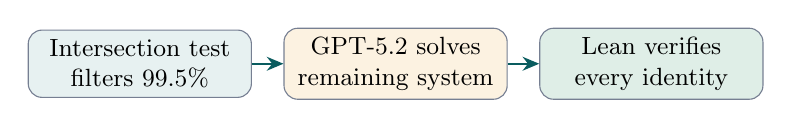
\begin{tikzpicture}
  \node[pipebox=Teal!10, text width=2.6cm, minimum height=0.7cm, font=\small]
    (int) {Intersection test\\filters 99.5\%};
  \node[pipebox=Amber!15, text width=2.6cm, minimum height=0.7cm, font=\small, right=0.4cm of int]
    (ai) {GPT-5.2 solves\\remaining system};
  \node[pipebox=Sage!15, text width=2.6cm, minimum height=0.7cm, font=\small, right=0.4cm of ai]
    (lean) {Lean verifies\\every identity};
  \draw[fatarr] (int) -- (ai);
  \draw[fatarr] (ai) -- (lean);
\end{tikzpicture}
\end{center}
\end{frame}

% =====================================================================
% Slide: Intersection Test — Why It Works
% =====================================================================
\begin{frame}{Why Most KL Constraints Vanish}

$\braket{0_L|P|0_L}$ sums over pairs where
$x$ and $x \oplus z_P$ are \emph{both} in $S_0$.

\begin{center}
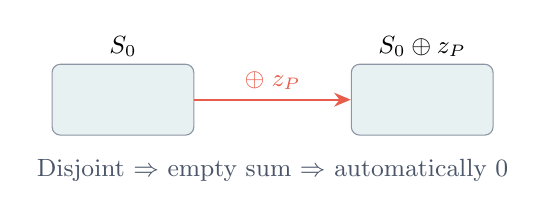
\begin{tikzpicture}[
  sset/.style={draw=Navy!50, rounded corners=3pt, minimum width=1.8cm,
    minimum height=0.9cm, fill=#1},
]
  \node[sset=Teal!10] (s0) at (0,0) {};
  \node[above=-1pt] at (s0.north) {\small $S_0$};
  \node[sset=Teal!10] (s0x) at (3.8,0) {};
  \node[above=-1pt] at (s0x.north) {\small $S_0 \oplus z_P$};
  \draw[fatarr, Coral] (s0.east) -- node[above, font=\small]{$\oplus\; z_P$} (s0x.west);
  \node[font=\small, text=Slate] at (1.9,-0.9) {Disjoint $\Rightarrow$ empty sum $\Rightarrow$ automatically $0$};
\end{tikzpicture}
\end{center}

\vspace{-0.5em}
$S_0 \cap (S_0 \oplus z_P) = \emptyset
  \;\Longrightarrow\; \braket{0_L|P|0_L} = 0$.

\begin{exampleblock}{Why so effective}
$S_0$ is \textbf{sparse}: $|S_0| = 7$ out of $2^7 = 128$.
Random shifts almost never land back inside $S_0$.\;
Only \alert{25}\,/\,49,152 survive (BD16v1).
\end{exampleblock}

In Lean: \code{klIsAutomatic} is \code{Decidable} --- checked by \code{native\_decide}.
\end{frame}

% =====================================================================
% Slide: GPT-5.2 Discovers Solutions
% =====================================================================
\begin{frame}{From Constraints to Solutions: GPT-5.2}

After intersection test, $\sim$25--150 surviving constraints form a
\textbf{quadratic system} in $c_x \in \CC$.

\begin{columns}[T]
\column{0.48\textwidth}
\textbf{The problem}:
\begin{itemize}\setlength\itemsep{0pt}
\item Unknowns: $c_x$ for each $x \in S_0$
\item $\sum_{x} \bar{c}_x\, c_{x'}\!\cdot\!(\text{phase}) = 0$
\item Non-convex $\Rightarrow$ hard for standard solvers
\end{itemize}

\column{0.48\textwidth}
\textbf{GPT-5.2's approach}:
\begin{itemize}\setlength\itemsep{0pt}
\item Given $S_0$, probabilities, constraint eqns
\item Exploits symmetries, groups terms
\item Returns \textbf{closed-form} amplitudes
  in $\QQ(\sqrt{2},\sqrt{3},i)$
\end{itemize}
\end{columns}

\vspace{0.2em}
\begin{center}
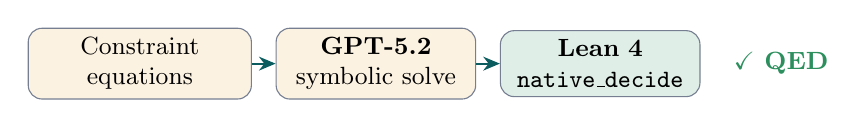
\begin{tikzpicture}
  \node[pipebox=Amber!15, text width=2.6cm, minimum height=0.6cm, font=\small]
    (c) {Constraint\\equations};
  \node[pipebox=Amber!15, text width=2.3cm, minimum height=0.6cm, font=\small, right=0.3cm of c]
    (ai) {\textbf{GPT-5.2}\\symbolic solve};
  \node[pipebox=Sage!15, text width=2.3cm, minimum height=0.6cm, font=\small, right=0.3cm of ai]
    (lean) {\textbf{Lean 4}\\\code{native\_decide}};
  \node[right=0.3cm of lean, font=\small\bfseries, text=Sage] {$\checkmark$ QED};
  \draw[fatarr] (c) -- (ai);
  \draw[fatarr] (ai) -- (lean);
\end{tikzpicture}
\end{center}
\end{frame}

% =====================================================================
% Slide: Exact Arithmetic
% =====================================================================
\begin{frame}{Exact Arithmetic in $\QQ(\sqrt{2},\sqrt{3},\,i)$}

$m{=}8 \Rightarrow \omega_8 = \tfrac{1+i}{\sqrt{2}}$.\;
Amplitudes involve $\sqrt{2}$, $\sqrt{3}$ from normalization.

\begin{columns}[T]
\column{0.48\textwidth}
\begin{block}{Representation (\code{QSqrt23i})}
Each element $= (q_0,\ldots,q_7)\in\QQ^8$:
{\small\[
  (q_0 {+} q_1\sqrt{2} {+} q_2\sqrt{3} {+} q_3\sqrt{6})
  + (\cdots)\,i
\]}
\end{block}

Multiplication closed.\\
Equality \emph{decidable} (rational coefficients).

\column{0.48\textwidth}
\begin{exampleblock}{BD16v1 amplitudes (GPT-5.2)}
{\small
\begin{tabular}{@{}ll@{}}
$c_0 {=} \tfrac{1}{4}$ & $c_5 {=} \tfrac{1}{4}$\\[2pt]
$c_1 {=} c_2 {=} \tfrac{\sqrt{3}}{4}$ & $c_6 {=} \tfrac{i}{2}$\\[2pt]
$c_3 {=} c_4 {=} \tfrac{\sqrt{2}}{4}$\\
\end{tabular}
}

In Lean: $c_1 = (0,0,\tfrac{1}{4},0,\;0,0,0,0)$\;\chk
\end{exampleblock}
\end{columns}

\vspace{0.2em}
\textcolor{Slate}{\small No floating point.  Every operation exact over $\QQ$.
\code{DecidableEq} $\Rightarrow$ \code{native\_decide} verifies each KL identity.}
\end{frame}

% =====================================================================
% Slide: Two-Layer Verification
% =====================================================================
\begin{frame}{Two-Layer Verification Architecture}

\begin{center}
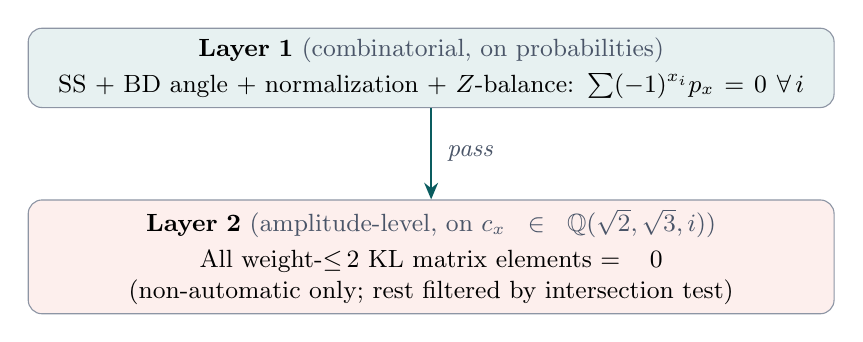
\begin{tikzpicture}[
  lbox/.style={draw=Navy!50, rounded corners=5pt, text width=10cm,
    align=center, font=\small, minimum height=1cm},
]
  \node[lbox, fill=Teal!10] (l1) at (0,0)
    {\textbf{Layer 1} \textcolor{Slate}{(combinatorial, on probabilities)}\\[2pt]
     SS $+$ BD angle $+$ normalization $+$
     $Z$-balance: $\sum(-1)^{x_i}p_x = 0\;\forall\,i$};
  \node[lbox, fill=Coral!10] (l2) at (0,-2.4)
    {\textbf{Layer 2} \textcolor{Slate}{(amplitude-level, on $c_x \in \QQ(\sqrt{2},\sqrt{3},i)$)}\\[2pt]
     All weight-${\leq}\,2$ KL matrix elements $= 0$\\
     (non-automatic only; rest filtered by intersection test)};

  \draw[fatarr] (l1) -- node[right, font=\small\itshape, text=Slate, xshift=2pt]{pass} (l2);
\end{tikzpicture}
\end{center}

\vspace{0.5em}
Both layers are \textbf{fully decidable} --- verified by \code{native\_decide}.

No \code{sorry}, no axioms. Build time per code: 2--11\,s.
\end{frame}

% =====================================================================
% Slide: BD16v1 Detailed Example
% =====================================================================
\begin{frame}[fragile]{BD16 Example: $((7,2,3))$ with $\mathbf{a}=(1,2,2,2,2,3,3)$}

$m{=}8$ (transversal $T$),\;
$|S_0| = 7$.\quad
{\small
$4\ket{0_L}
  {=}
  \ket{0000000}
  {+}\sqrt{3}\ket{0111100}
  {+}\sqrt{3}\ket{1001110}
  {+}\sqrt{2}\ket{1010101}
  {+}\sqrt{2}\ket{1011001}
  {+}\ket{1110010}
  {+}2i\ket{0100011}$
}

\vspace{0.2em}
\begin{columns}[T]
\column{0.56\textwidth}
\begin{lstlisting}[style=lean,basicstyle=\ttfamily\scriptsize]
def bd16Data : Distance3Data 7 8 where
  a    := ![1, 2, 2, 2, 2, 3, 3]
  b₀   := 0
  supp₀ := {s0, s1, s2, s3, s4, s5, s6}
  prob₀ := ... -- (1,3,3,2,2,1,4)/16

theorem layer1 : bd16Data.Layer1OK
  := by native_decide
theorem layer2 : AllKLSatisfied supp₀ amp₀ 2
  := by native_decide
\end{lstlisting}

\column{0.40\textwidth}
{\small
\begin{tabular}{@{}ll@{}}
\toprule
\textbf{Check} & \textbf{Result} \\
\midrule
SS + BD + norm & \leanproof \\
$Z$-balance & \leanproof \\
Non-auto KL & 25 / 49152 \\
All 25 $= 0$ & \leanproof \\
\bottomrule
\end{tabular}
}

\vspace{0.3em}
\tikz\node[draw=Sage, fill=Sage!6, rounded corners=3pt, inner sep=4pt, text width=3.4cm, align=center, font=\small]{%
  \textbf{Complete $d{\geq}3$ proof}\\Build: 2.6\,s};
\end{columns}
\end{frame}

% =====================================================================
% Slide: All 8 BD16 Codes
% =====================================================================
\begin{frame}{8 Verified BD16 $((7,2,3))$ Codes}

All codes: $n{=}7$, $K{=}2$, $m{=}8$ (transversal $T$), 
verified \code{Layer1OK} $+$ \code{AllKLSatisfied}.

\vspace{0.2em}
\begin{center}
{\footnotesize
\begin{tabular}{@{}llccll@{}}
\toprule
\textbf{File} & \textbf{Angle vector $\mathbf{a}$} & $|S_0|$ & $\lambda^*$ & \textbf{Solution type} & \textbf{Status} \\
\midrule
\code{BD16v1}  & $(1,2,2,2,2,3,3)$ & 7  & $\sqrt{21/8}$ & 2-param continuous  & \leanproof \\
\code{BD16v2}  & $(1,1,2,2,2,2,5)$ & 10 & $\sqrt{33}/4$ & 192-elt discrete & \leanproof \\
\code{BD16v3a} & $(0,1,2,2,3,3,4)$ & 7  & $\sqrt{51}/4$ & Solution A (of 3)   & \leanproof \\
\code{BD16v3b} & $(0,1,2,2,3,3,4)$ & 8  & $\sqrt{23}/4$ & Solution B (of 3)   & \leanproof \\
\code{BD16v3c} & $(0,1,2,2,3,3,4)$ & 8  & $\sqrt{30}/4$ & Solution C (of 3)   & \leanproof \\
\code{BD16v4}  & $(1,1,1,1,3,3,5)$ & 13 & $\sqrt{177}/8$ & continuous          & \leanproof \\
\code{BD16v5}  & $(1,1,1,1,3,4,4)$ & 12 & $\sqrt{62}/4$ & 128-elt discrete & \leanproof \\
\code{BD16v6a} & $(1,1,1,2,2,4,4)$ & 16 & $1$           & uniform magnitude   & \leanproof \\
\bottomrule
\end{tabular}
}
\end{center}

\textcolor{Slate}{\small
Remaining: 3 vectors need $\sqrt{10}$ (field extension); 2 proven impossible.
12 vectors total $\Rightarrow$ 10 feasible, 8 verified.
}
\end{frame}

% =====================================================================
% Slide: Non-Automatic Constraints in Detail
% =====================================================================
\begin{frame}{What the Surviving Constraints Look Like}

After the intersection test, ${\sim}25$--$150$ non-automatic Pauli strings remain.

\begin{columns}[T]
\column{0.48\textwidth}
\begin{block}{Diagonal ($Z_iZ_j$)}
$\braket{0_L|Z_iZ_j|0_L} = \sum_{x \in S_0} (-1)^{x_i+x_j}\,|c_x|^2$

\emph{Linear} in probabilities $p_x = |c_x|^2$.\\
Already verified in \textbf{Layer~1}.
\end{block}

\begin{exampleblock}{Key simplification}
BD symmetry $\ket{1_L} = X^{\otimes n}\ket{0_L}$\\
$\Rightarrow$ off-diagonal eqns \textbf{pair up}:\\
$\braket{0|P|0} = 0 \Leftrightarrow \braket{1|P|1} = 0$

Only $\ket{0_L}$ amplitudes needed.
\end{exampleblock}

\column{0.48\textwidth}
\begin{alertblock}{Off-diagonal ($X_iX_j, X_iY_j, \ldots$)}
$\braket{0_L|P|0_L} = \displaystyle\sum_{\substack{x \in S_0 \\ x \oplus z_P \in S_0}}
  \bar{c}_x\, c_{x \oplus z_P}\, \omega^{f(x,P)}$

\emph{Quadratic} in amplitudes $c_x \in \CC$.\\
Phases $\omega^{f(x,P)}$ depend on $x_P$ bits.
\end{alertblock}

\textcolor{Slate}{\small BD16v1 ($|S_0|{=}7$): 25 constraints $\to$ 7 complex unknowns with 1 normalization $+$ 7 probability values fixed.}
\end{columns}
\end{frame}

% =====================================================================
% Slide: Solution Landscape
% =====================================================================
\begin{frame}{The BD$_{16}$ Solution Landscape}

All 12 BD$_{16}$ $((7,2,3))$ angle vectors (up to qubit permutation, $a_i \leftrightarrow m{-}a_i$):

\vspace{-0.3em}
\begin{center}
{\scriptsize
\begin{tabular}{@{}lcccl@{}}
\toprule
\textbf{Angle vector $\mathbf{a}$} & $|S_0|$ & \textbf{Non-auto} & \textbf{Solution type} & \textbf{Status} \\
\midrule
$(1,2,2,2,2,3,3)$ & 7  & 25  & 2-param continuous & \textcolor{Sage}{Lean \checkmark} \\
$(1,1,2,2,2,2,5)$ & 10 & 94  & discrete family    & \textcolor{Sage}{Lean \checkmark} \\
$(0,1,2,2,3,3,4)$ & 7  & 47  & 3 isolated solutions & \textcolor{Sage}{Lean \checkmark} \\
$(1,1,1,1,3,3,5)$ & 13 & 145 & continuous          & \textcolor{Sage}{Lean \checkmark} \\
$(1,1,1,1,3,4,4)$ & 12 & 112 & discrete family    & \textcolor{Sage}{Lean \checkmark} \\
$(1,1,1,2,2,4,4)$ & 16 & 149 & uniform magnitude  & \textcolor{Sage}{Lean \checkmark} \\
\rowcolor{Amber!10}
$(1,1,2,2,3,3,3)$ & 14 & 134 & needs $\sqrt{10}$  & \textcolor{Amber}{pending} \\
\rowcolor{Amber!10}
$(1,1,1,2,3,3,4)$ & 12 & 103 & needs $\sqrt{10}$  & \textcolor{Amber}{pending} \\
\rowcolor{Amber!10}
$(1,1,1,2,2,3,5)$ & 10 & 86  & needs $\sqrt{10}$  & \textcolor{Amber}{pending} \\
\rowcolor{Coral!8}
$(1,1,2,2,2,6,1)$ & 5  & 11  & \multicolumn{2}{l}{\textcolor{Coral}{proven infeasible}} \\
\rowcolor{Coral!8}
$(0,1,1,2,3,3,5)$ & 4  & 4   & \multicolumn{2}{l}{\textcolor{Coral}{proven infeasible}} \\
$(0,0,1,2,3,3,6)$ & 4  & 2   & numerical only & \textcolor{Slate}{unresolved} \\
\bottomrule
\end{tabular}
}
\end{center}

\vspace{-0.5em}
\textcolor{Slate}{\small 8/10 feasible vectors verified.\ 3 pending need $\QQ(\sqrt{2},\sqrt{3},\sqrt{5},i)$ (16-dim field).}
\end{frame}

% =====================================================================
\section{Outlook}
% =====================================================================

% =====================================================================
% Slide: Batch Verification
% =====================================================================
\begin{frame}{Outlook: Batch Verification of All 14,116 Codes}

The distance-2 catalogue has 14,116 $((n,K,2))$ codes.  Currently: individual
Lean files for representative examples.

\begin{columns}[T]
\column{0.50\textwidth}
\begin{block}{Scaling strategy}
\begin{enumerate}\setlength\itemsep{0pt}
\item Python exports each code's data as a \code{.lean} file
  (support, probabilities, angle vector)
\item Lean's \code{ExampleData.OK} bundle checks
  SS $+$ screen $+$ normalization $+$ $Z$-KL
\item \code{native\_decide} proves each in $< 1$\,s
\item \code{lake build} compiles all 14K files
\end{enumerate}
\end{block}

\column{0.46\textwidth}
\begin{exampleblock}{Already demonstrated}
\begin{itemize}\setlength\itemsep{0pt}
\item \code{Ex522.lean}, \code{Ex622.lean}:\\
  fully verified via \code{native\_decide}
\item Build time: 0.3--0.8\,s each
\item At 1\,s/code: $\sim$4 hours total\\
  (embarrassingly parallel)
\end{itemize}
\end{exampleblock}

\tikz\node[draw=Teal!60, fill=Teal!6, rounded corners=3pt, inner sep=4pt,
  text width=4cm, align=center, font=\small]{%
  \textbf{14,116 machine-checked}\\
  \textbf{proofs}: within reach};
\end{columns}
\end{frame}

% =====================================================================
% Slide: Family II and Higher Analytical Families
% =====================================================================
\begin{frame}{Outlook: Analytical Family~II \& Beyond}

\vspace{-0.2em}
\begin{columns}[T]
\column{0.48\textwidth}
\begin{block}{Family II: 4-element support}
$C_0 = \{0^n, 1^n, e_1 \bar{e}_1, \bar{e}_1 e_1 \}$

Free parameter $\lambda \in [0,1]$ $\to$ continuous family.

Lean: \code{familyII\_OK}\;
$\forall\,(n,m,s,\lambda)$ passing screens.
\end{block}

\begin{alertblock}{$\lambda$-Families A--E (verified)}
5 families at $n{=}5$, each covers $\infty$ values.\\
$\Sigma_Z(\lambda) = \sum_i \braket{Z_i}^2 \in [\tfrac{1}{3},\,1]$
\end{alertblock}

\column{0.48\textwidth}
\begin{exampleblock}{What universality buys}
\begin{itemize}\setlength\itemsep{0pt}
\item One 100-line file $\to$ \textbf{all} instantiations
\item Proves \textbf{structure}, not cases
\item Classification complete for $|C_0| \leq 4$
\end{itemize}
\end{exampleblock}

\textbf{Open}: analytical families for \alert{distance 3}?

\textcolor{Slate}{\small Needs universal proofs over $\QQ(\sqrt{\cdot},i)$
with amplitude parameters --- significantly harder.}
\end{columns}
\end{frame}

% =====================================================================
% Slide: Beyond BD16
% =====================================================================
\begin{frame}{Outlook: Beyond BD$_{16}$}

BD$_{16}$ at $n{=}7$ is the \textbf{first step}.\; The framework extends naturally:

\vspace{-0.2em}
\begin{columns}[T]
\column{0.31\textwidth}
\begin{block}{Other BD groups}
BD$_{12}$--BD$_{36}$ ($m{=}6$--$18$)

Same pipeline; number field adapts to $\omega_m$.

\textcolor{Slate}{\small Zhang--Zeng: dozens of $((7,2,3))$ candidates}
\end{block}

\column{0.31\textwidth}
\begin{alertblock}{$n{=}8$: $T^{1/4}$}
BD$_{64}$ ($m{=}32$):\\
transversal $\pi/16$.

Intersection test still filters $>99\%$ of KL.
\end{alertblock}

\column{0.31\textwidth}
\begin{exampleblock}{Exceptional groups}
$2I$ ($|G|{=}120$): 5th level\\
$2T$ ($|G|{=}24$)\\
$2O$ ($|G|{=}48$)

Two-layer architecture still applies.
\end{exampleblock}
\end{columns}

\vspace{0.3em}
\begin{center}
\tikz\node[draw=Navy!40, fill=Navy!4, rounded corners=4pt, inner sep=5pt,
  text width=11cm, align=center, font=\small]{%
  \textbf{Long-term vision}: a formal library of quantum codes
  with \textbf{machine-verified} fault-tolerance properties ---
  AI discovers, Lean certifies.};
\end{center}
\end{frame}

% =====================================================================
\section{Summary}
% =====================================================================

% =====================================================================
% Slide: Summary
% =====================================================================
\begin{frame}{Summary}

\begin{columns}[T]
\column{0.48\textwidth}
\begin{block}{Distance 2}
\begin{itemize}\setlength\itemsep{0pt}
\item Full SSLP pipeline in Lean 4
\item Residue-shift screen $\Rightarrow$ $d{\geq}2$ automatic
\item 14,116 codes certified
\item Analytical families: one proof $\to \infty$ codes
\end{itemize}
\end{block}

\begin{exampleblock}{Codebase}
${\sim}$4,300 lines Lean 4,\; 0 \code{sorry}\\
\code{github.com/LionSR/lean-qec}
\end{exampleblock}

\column{0.48\textwidth}
\begin{block}{Distance 3 (new)}
\begin{itemize}\setlength\itemsep{0pt}
\item Intersection test filters 99.5\%
\item GPT-5.2 $\to$ closed-form amplitudes
\item Exact arithmetic in $\QQ(\sqrt{2},\sqrt{3},i)$
\item 8 BD$_{16}$ $((7,2,3))$ codes: first\\
  machine-checked $d{=}3$ proofs
\end{itemize}
\end{block}

\begin{alertblock}{What's next}
Batch 14K codes\; $\cdot$\; $\QQ(\sqrt{5})$ extension\; $\cdot$\;
BD$_{12}$--BD$_{36}$\; $\cdot$\; $n{=}8$\; $\cdot$\; 2I/2T/2O
\end{alertblock}
\end{columns}
\end{frame}

% =====================================================================
% CLOSING
% =====================================================================
{
\setbeamercolor{background canvas}{bg=Navy}
\begin{frame}[standout]
  \textcolor{white}{\large Thank you}\\
  \textcolor{Ice}{\normalsize
    arXiv:2510.20728 \quad·\quad
    \texttt{github.com/LionSR/lean-qec}}
\end{frame}
}

\end{document}